\documentclass[conference]{IEEEtran}
\IEEEoverridecommandlockouts
% The preceding line is only needed to identify funding in the first footnote. If that is unneeded, please comment it out.
\usepackage{cite}
\usepackage[ngerman]{babel}
\usepackage[utf8]{inputenc}
\usepackage{amsmath,amssymb,amsfonts}
\usepackage{algorithmic}
\usepackage{graphicx}
\usepackage{textcomp}
\usepackage{xcolor}
\usepackage{listings}


\definecolor{pblue}{rgb}{0.13,0.13,1}
\definecolor{pgreen}{rgb}{0,0.5,0}
\definecolor{pred}{rgb}{0.9,0,0}
\definecolor{pgrey}{rgb}{0.46,0.45,0.48}
\lstset{language=Java,
	showspaces=false,
	showtabs=false,
	breaklines=true,
	tabsize=2,
	showstringspaces=false,
	breakatwhitespace=true,
	commentstyle=\color{pgreen},
	keywordstyle=\color{pblue},
	stringstyle=\color{pred},
	basicstyle=\ttfamily
}


\usepackage{url}
\def\BibTeX{{\rm B\kern-.05em{\sc i\kern-.025em b}\kern-.08em
		T\kern-.1667em\lower.7ex\hbox{E}\kern-.125emX}}
\begin{document}
	
	\title{Computational Geometry - Abgabe 3}
	
	\author{\IEEEauthorblockN{1\textsuperscript{st} Bartolovic Eduard}
		\IEEEauthorblockA{\textit{Hochschule München} \\
			München, Deutschland \\
			eduard.bartolovic0@hm.edu}
	}
	
	\maketitle
	
	%\begin{abstract}	
	%\end{abstract}

	\section{Basis Bentley-Ottmann Algorithmus}
	
	Zu Beginn werden alle Start und Endpunkte aller Strecken $L_{InputStrecken}$ in eine EventQueue $Q_{Event}$ eingefügt. Diese EventQueue ist eine PriorityQueue die intern die Events auf der X-Achse und Eventtyp sortiert. \textit{START} Events haben bei gleichem X Wert Vorrang. \textit{END} Events sind immer zuletzt dran. Die PriorityQueue ist als ein Heap implementiert. Die Operationen besitzen deshalb auch die Komplexität \cite{b2}:
	\begin{itemize}
		\item add: $\mathcal{O}(log(n))$
		\item poll: $\mathcal{O}(1)$
	\end{itemize}
	Relevante Strecken liegen in der Sweepline $T_{Sweep}$.
	Für die Sweepline $T_{Sweep}$ wird als Datenstruktur eine Baum basierend auf einer Rot-Schwarz-Baum Implementierung verwendet. Dieser hat die Komplexität \cite{b1}:
	\begin{itemize}
		\item add: $\mathcal{O}(log(n))$
		\item remove: $\mathcal{O}(log(n))$
		\item contains: $\mathcal{O}(log(n))$
		\item get: $\mathcal{O}(log(n))$
	\end{itemize}
	Es gibt im regulären Bentley-Ottmann Algorithmus 3 Events (\textit{START}, \textit{END}, \textit{INTERSECTION}).
	Zu beginn liegen nur \textit{START} und \textit{END} Events in $Q_{Event}$.\\
	Nun wird nacheinander ein Event aus $Q_{Event}$ genommen. Dieses Event wird je nach Typ behandelt.\\
	Das Event \textit{START} fügt das neue Segment $S_{new}$ in die Sweepline $T_{Sweep}$ ein.
	Es wird überprüft ob ein Segment über oder unter $S_{new}$ liegt. Sollte dies der Fall sein wird überprüft ob diese sich mit $S_{new}$ schneiden. Bei einem gefundenen Schnittpunkten wird ein neues \textit{INTERSECTION} Event in $T_{Sweep}$ eingefügt.\\
	Bei einem \textit{END} Event endet ein Segment $S_{old}$. Es wird überprüft ob ein Segment über und unter $S_{old}$ liegt. Sollten diese existieren dann wird überprüft ob diese sich schneiden. Bei einem gefundenen Schnittpunkten wird ein neues \textit{INTERSECTION} Event in $Q_{Event}$ eingefügt. $S_{old}$ wird aus der Sweepline $T_{Sweep}$ entfernt.\\
	Bei einem \textit{INTERSECTION} Event schneiden sich die zwei Segmente s und t. Dabei werden die Positionen von s und t in $T_{Sweep}$ getauscht. Nach dem werden die Segmente r und u, die möglicherweise unmittelbar unter bzw. über t und s liegen nach Schnittpunkten untersucht. Gefundene Schnittpunkte werden der Ereigniswarteschlange hinzugefügt.

	\section{Schnittpunkt zwischen 2 Geraden }
	Da es nicht reicht nur zu Wissen das zwei geraden einen Schnittpunkt haben sondern es auch nötig ist auch dessen genaue Position zu kennen musste ein neuer Algortithmus entwickelt werden.\\
	Hierfür wurde erstmal überprüft ob der Start- oder Endpunkt p1,q1 der Strecke s1 identisch zu einem der Punkt p2 oder q2 der Strecke s2 ist. Sollte dies der Fall sein wird direkt der gemeinsame Punkt zurückgegeben.\\
	Nun werden die beiden Strecken als Geraden behandelt. So kann man mit der Geradengleichung den Schnittpunkt der zwei Geraden berechnen.\\
	\[  \]
	Es besteht die Möglichkeit das der Schnittpunkt S nicht existiert da beide Geraden parallel zu einander sind. In diesem Fall wären wären x und y von S unendlich. In diesem Fall wird ein Optional.empty() zurückgegeben.
	Da der Schnittpunkt S über die Geradengleichung berechnet worden ist kann es sein das dieser sich auf den Geraden von s1 und s2 befindet aber nicht auf der Strecke s1 oder s2. Deshalb muss überprüft werden ob sich der Punkt in der Bounding Box der beiden Strecken befindet. Sollte dies bei beiden der Fall sein dann ist dies der korrekte Schnittpunkt.\\
	Um numerische Fehler zu reduzieren wird bei Horizontalen und Vertikalen Strecken ....
	++++++++++++++++++++++++++
	\section{Probleme für den Algoritmus}
	Der Algorithmus hat Probleme wenn folgende Voraussetzungen nicht erfüllt sind:
	\begin{enumerate}
		\item x-Koordinaten der Schnitt- und Endpunkte sind paarweise verschieden
		
		\item Länge der Segmente $> 0$
		
		\item nur echte Schnittpunkte
		
		\item keine Linien parallel zur y-Achse
		
		\item keine Mehrfachschnittpunkte
		
		\item keine überlappenden Segment
	\end{enumerate}
	
	\begin{figure}[h]
		\begin{center}
			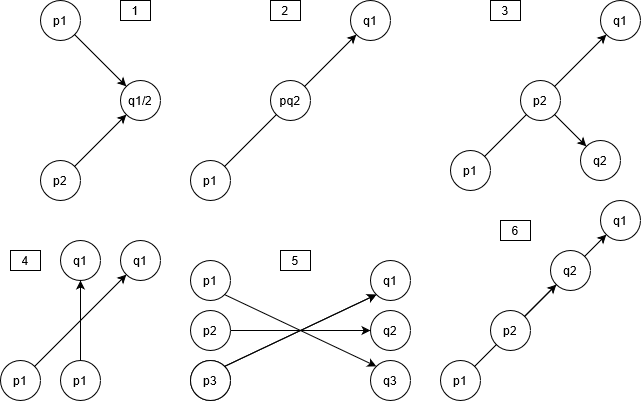
\includegraphics[width=6cm]{ProblemFaelle.png}
			\caption{Problemfälle für den Standard Bentley Ottman algorithmus}
			\label{figure_3}
		\end{center}
	\end{figure}



	\section{Behandlung der Sonderfälle}
	In meiner Implementierung werden alle Sonderfälle behandelt.
	\subsection{Nur echte Schnittpunkte}
	Meine Implementierung unterstützt auch unechte Schnittpunkte. Hierfür wurde vor allem die Sweepline angepasst. So wird die gewöhnliche Sweepline Implementierung die nur aus einem Baum $T_{Sweep}$ mit Strecken besteht mit einer Funktionalität ergänzt die ähnlich wie bei Buckets bei einem Hashset funktioniert. So wird bei START Events überprüft ob die Position des Startpunktes in $T_{Sweep}$ bereits existiert. Sollte dies der Fall sein wird das Segment einfach zusätzlich in den Knoten eingefügt. Der Schlüssel der Knoten ist der aktuelle Y-Wert.\\
	\begin{figure}[h!]
		\begin{center}
			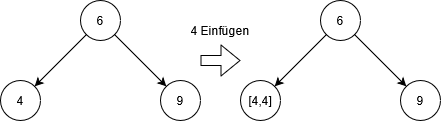
\includegraphics[width=6cm]{BaumKollision.png}
			\caption{Einfügen in die Sweepline mit Kollision}
			\label{figure_collision}
		\end{center}
	\end{figure}\\
	Leider müssen werden jedes mal wenn die Sweepline bewegt wird die Elemente in $T_{Sweep}$ zu neu sortiert werden. $T_{Sweep}$ neu zu sortieren bedarf $\mathcal{O}(n*log(n))$. Theoretisch müsste es möglich sein dies zu vermeiden in dem immer nur die Nachbar verglichen werden. Dies ist aber sehr komplex da bei Neusortierungen die Buckets mit neu sortiert werden müssen. Ich bin überzeugt das es auch ohne kompletter Neusortierung gehen müsste. Der Aufwand dafür ist aber extrem hoch. Es reicht nicht aus immer nur die direkten Nachbarn zu betrachten da potentiell weiter entfernte Strecken auch noch in Betracht kommen können. Deshalb muss neben den direkten Nachbarn noch weiter überprüft werden bis man sicher gehen kann das diese sich nicht schneiden können.
	
	\subsection{X-Koordinaten der Schnitt- und Endpunkte sind paarweise identisch}
	Dieses Problem ist ein Teilproblem des vorherigen Problems und damit schon gelöst.
	So wird beim einfügen neuer Strecken überprüft ob bereits andere Segmente an diesem Punkt liegen. Sollte dies der Fall sein werden wird dieser Punkt entsprechend der Anzahl der Segmente als Schnittpunkte in die Output Liste eingefügt. Außerdem immer wenn ein Schnittpunkt gefunden wird welcher direkt auf der Sweepline $T_{Sweep}$ liegt wird dieser ohne ein \textit{INTERSECTION} Event zu generieren der Outputliste hinzugefügt.
	
	\subsection{Linien parallel zur Y-Achse}
	Für Linien die zur Y-Achse gehören wurden in ein neues \textit{VERTICALLINE} Event erschaffen. So werden keine \textit{Start} und \textit{END} Event in die Eventqueue $Q_{Event}$ eingefügt sondern nur das \textit{VERTICALLINE} Event.
	Vertikale Strecken schneiden sich mit allen Strecken, die aktuell die Sweepline zwischen dem Start- und Endpunkt der vertikalen Strecke schneiden. So muss nicht die gesamte Sweepline $T_{Sweep}$ untersucht werden sondern nur ein Teilbaum.
	\begin{figure}[h]
		\begin{center}
			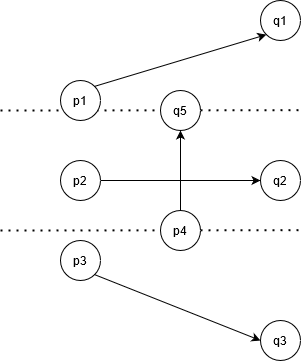
\includegraphics[width=6cm]{Vertikal.png}
			\caption{Suche nach Schnittpunkten mit Vertikalen Strecken in einem eingeschränkten Bereich}
			\label{figure_3}
		\end{center}
	\end{figure}
	Das gilt selbstverständlich auch für anderen Vertikalen Strecken an aktueller X-Stelle. Deshalb wird eine vertikale Strecke auch an einem \textit{VERTICALLINE} Event in die Sweepline $T_{Sweep}$ eingefügt. Sie werden aber nicht in den Baum eingefügt sondern in eine separate Liste für vertikale Segmente. Sobald die Sweepline verschoben wird werden alle vertikalen Strecken aus der Liste entfernt.
		
	\subsection{Länge der Segmente gleich $0$}
	Elemente der Länge 0 werden einfach als vertikale Segmente behandelt.
	
	\subsection{Mehrfachschnittpunkte}
	Mehrfachschnittpunkte wurden behandelt. Hierfür wird die oben beschriebene Baumstruktur der Sweepline $T_{Sweep}$ genutzt. So wird an einem \textit{INTERSECTION} Event in der SweepLine gesucht ob an der Stelle weitere Segmente durchlaufen. Sollte dies der Fall sein wird werden direkt die korrekte menge an Schnittpunkten der Outputliste hinzugefügt. Wichtig ist aber das der Fall in der Abbildung \ref{Multi} betrachtet wird. Hier muss an dem Schnittpunkt der höchste und niedrigste Segment gefunden werden und mit den benachbarten Strecken abgeglichen werden.
	\begin{figure}[h]
		\begin{center}
			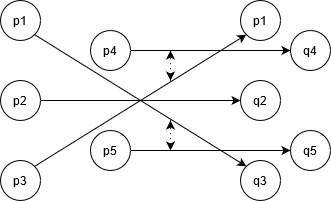
\includegraphics[width=6cm]{MultiSchnitt.png}
			\caption{Problemfälle mit überlappenden Elementen}
			\label{Multi}
		\end{center}
	\end{figure}
	
	\subsection{Überlappende Segmente}
	Auch dieses Problem ist auch ein Teilproblem der nur echten Schnittpunkte. Dies kann aber noch mehr Probleme bereiten als das nur Überlappungen in einzelnen Punkten. Wichtig ist das die Funktion die Schnittpunkte zwischen 2 Strecken findet in der Lage ist trotz Überlappung einen Schnittpunkt findet. Da eigentlich überlappende Segmente unendlich viele Schnittpunkte hat wird einfach der untere linke Punkt gewählt.\\
	Die wichtigsten Fälle sind in Abbildung \ref{figure_collision} abgebildet:
	\begin{figure}[h]
		\begin{center}
			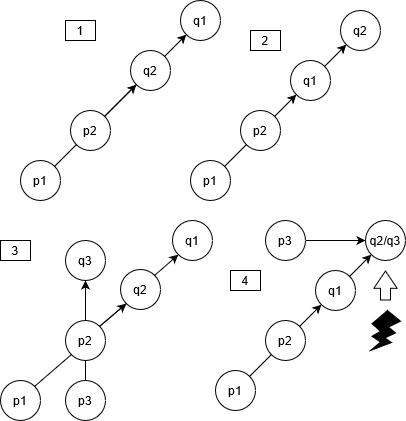
\includegraphics[width=6cm]{ProblemUberlappen.png}
			\caption{Problemfälle mit überlappenden Elementen}
			\label{figure_3}
		\end{center}
	\end{figure}\\
	Schwierig ist vor allem der Fall 4. Hier muss am Startpunkt $p3$ der Schnittpunkt $q2/q3$ gefunden werden. Dazu müssen die Strecken 1 und 2 welche beide gleich weit unter Strecke 3 liegen überprüft werden.
	
	\section{Genauigkeit}
	Ein Problem des Bentley Ottmann Verfahrens ist es das Schnittpunkte die sehr nah aneinander liegen Probleme verursachen können. Wichtig ist das die Berechnungen eine hohe Genauigkeit aufweisen. So liegen Schnittpunkte teilweise nur 4 Nachkommastellen auseinander.
	\begin{figure}[h]
		\begin{center}
			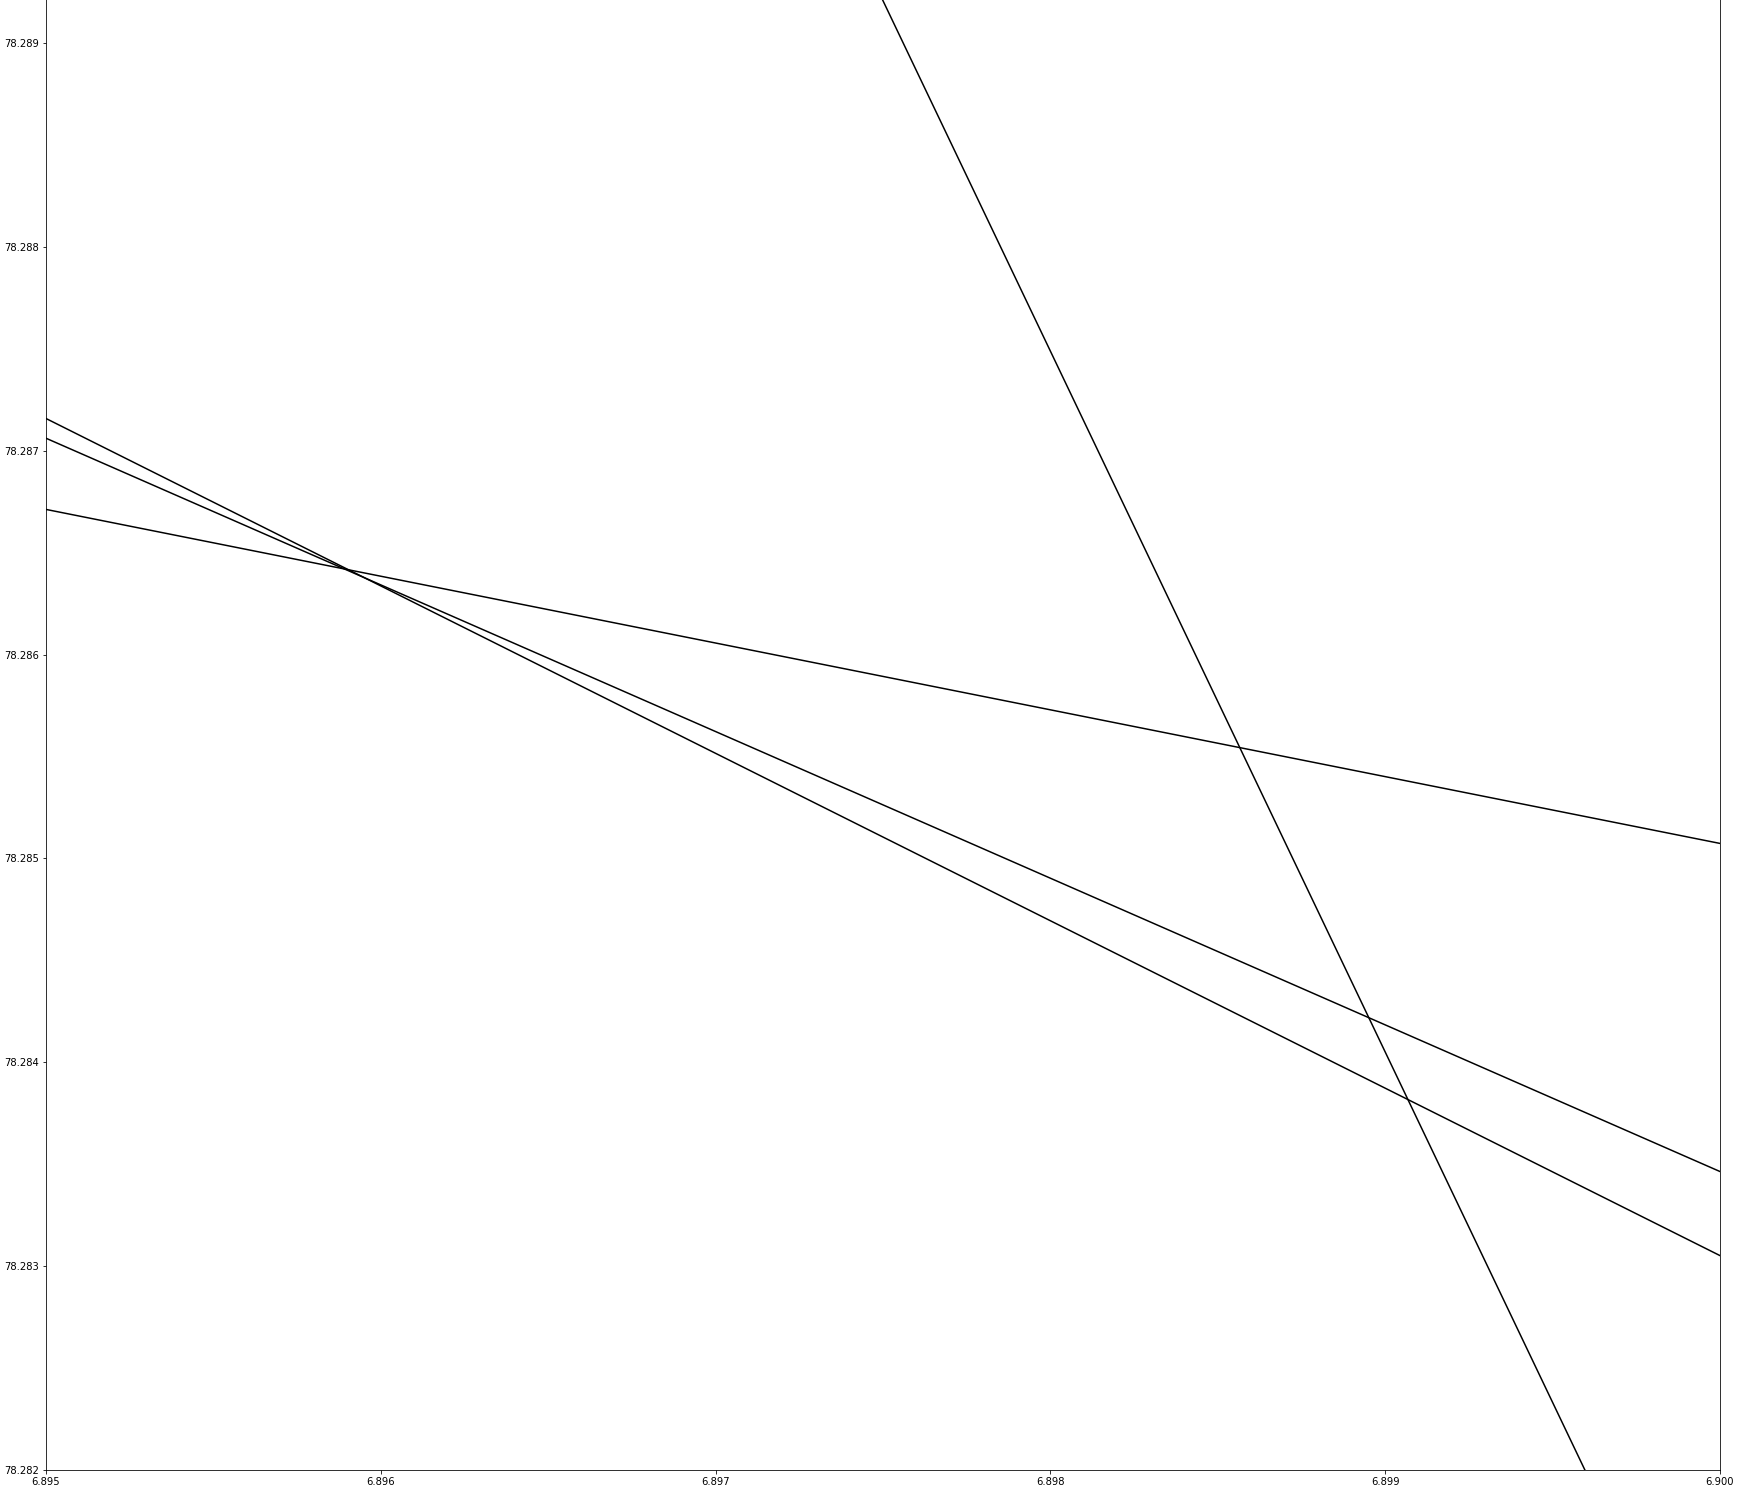
\includegraphics[width=6cm]{CloseIntersections.png}
			\caption{Sehr nah liegende Schnittpunkte}
			\label{figure_3}
		\end{center}
	\end{figure}\\
	\section{Komplexität}
	Die Komplexität ist abhängig vom Input. So gibt es normalerweise $2n + k$ Events, wobei $n$ die Anzahl der Segmente und $k$ die Anzahl der Schnittpunkten entspricht. Wobei bei Sonderfälle die Anzahl geringer Ausfallen kann. Da bei vertikalen Strecken nur ein Punkt in die Eventqueue eingefügt wird. Das selbe gilt auch für Schnittpunkte die in einem Startpunkt liegen und keinen neuen Eintrag in die EventQueue bekommen. So gilt für $m$ nicht vertikale Strecken, $s$ Schnittpunkte ohne Überschneidungen mit anderen Events und $v$ vertikalen Strecken:
	\[ 2n + k \geq 2m + s + v \]
	Die Komplexität des Sortierens der Eventqueue beträgt $\mathcal{O}((2m+v)*log(2m+v))$ was trotzdem $\mathcal{O}(n*log(n))$ entspricht.\\
	Operationen in die EventQueue und der Sweepline haben die Komplexität $\mathcal{O}(log(m))$. Allerdings wird bei jedem bewegen der Sweepline die Sweepline neu berechnet. Dies resultiert leider in $\mathcal{O}(m*log(m))$.\\
	Zusammengefasst kann man den Aufwand wie folgt beschreiben:
	\[\mathcal{O}(m*log(m)) + m*\mathcal{O}(m*log(m)) \]
	
	\newpage
	
	\section{Performance}
	
	\begin{enumerate}
		\item \textbf{BF S C:} BruteForce, SingleThread, nur Anzahl Schnittpunkte
		\item \textbf{BF S L:} BruteForce, SingleThread, Liste von Schnittpunkten
		\item \textbf{BF P C:} BruteForce, MultiThread, nur Anzahl Schnittpunkte
		\item \textbf{BF P L:} BruteForce, MultiThread, Liste von Schnittpunkten
		\item \textbf{BO:} Bentley-Ottmann, Liste von Schnittpunkten
	\end{enumerate}
     
	\begin{table}
		\small
		\begin{tabular}{|c|c|c|c|c|c|c|}
			\hline
			Datei & BF S C & BF S L & BF P C & BF P L & BO \\
			\hline
			s\_1000\_1 & 18 & 20 & 37 & 57 & 57\\
			\hline
			s\_1000\_10 & 13 & 13 & 1 & 2 & 14\\
			\hline
			s\_10000\_1 & 1263 & 1423 & 136 & 128 & 43\\
			\hline
			s\_100000\_1 & 111624 & 121718 & 8712 & 8825 & 45893\\%37363
			\hline
		\end{tabular}
	    \caption{Laufzeiten der Algorithmen}
	\end{table}

	Auch noch test mit 4Kerner?

	
	\section{Durchschnittliche Sweeplinegröße}
	Die durchschnittliche Füllgrad und die Anzahl der Verschiebungen der Sweepline beeinflusst die Performance maßgeblich. Die Anzahl der Schnittpunkte beeinflusst meistens auch die Anzahl der Verschiebungen der Sweepline. Dies kann man gut sehen wenn man die Zeiten in der oberen Tabelle mit der Abbildung \ref{fullstand} vergleicht. 

	\begin{figure}[!tbp]
		\centering
		\begin{minipage}[b]{0.5\textwidth}
			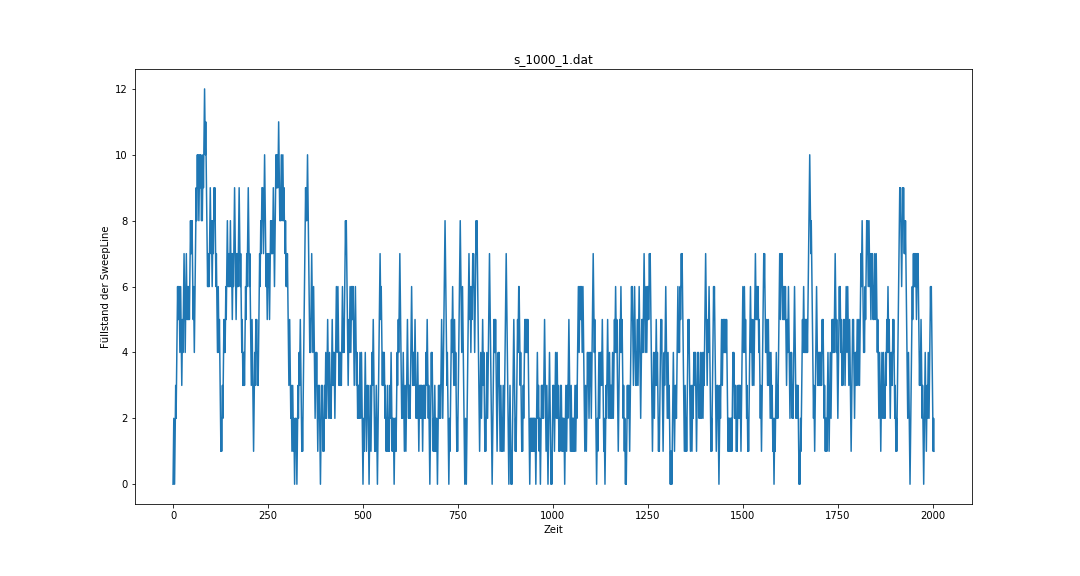
\includegraphics[width=\textwidth]{s1000+1.png}
		\end{minipage}
		\hfill
		\begin{minipage}[b]{0.5\textwidth}
			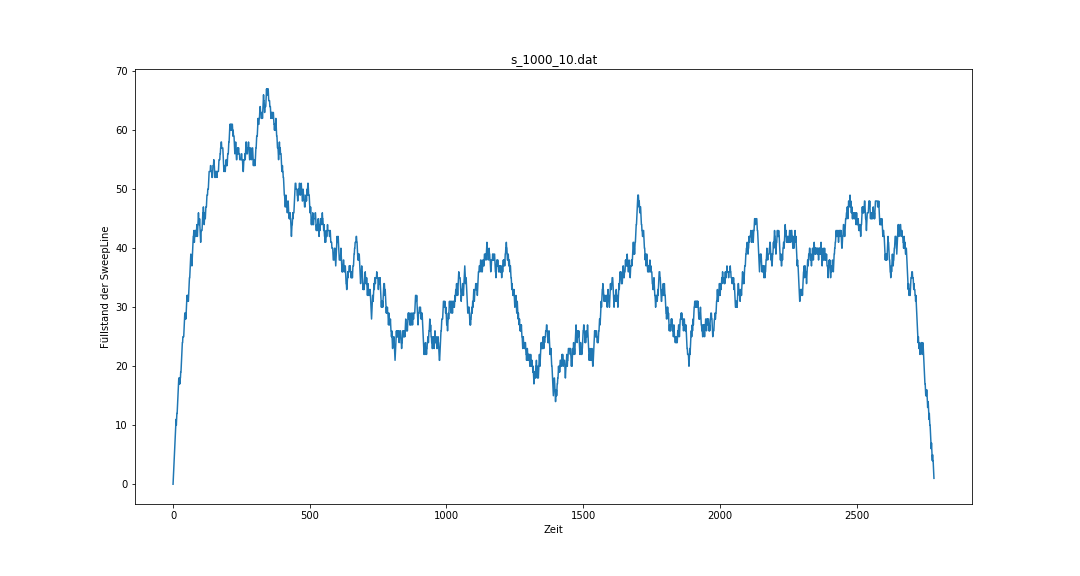
\includegraphics[width=\textwidth]{s1000+10.png}
		\end{minipage}
		\hfill
		\begin{minipage}[b]{0.5\textwidth}
			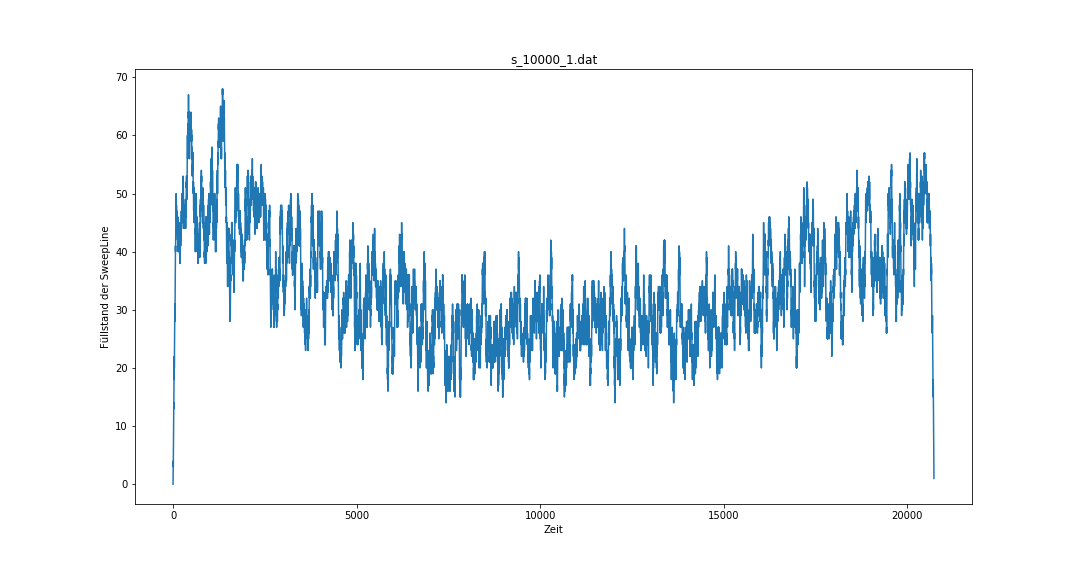
\includegraphics[width=\textwidth]{s10000+1.png}
		\end{minipage}
			\hfill
		\begin{minipage}[b]{0.5\textwidth}
			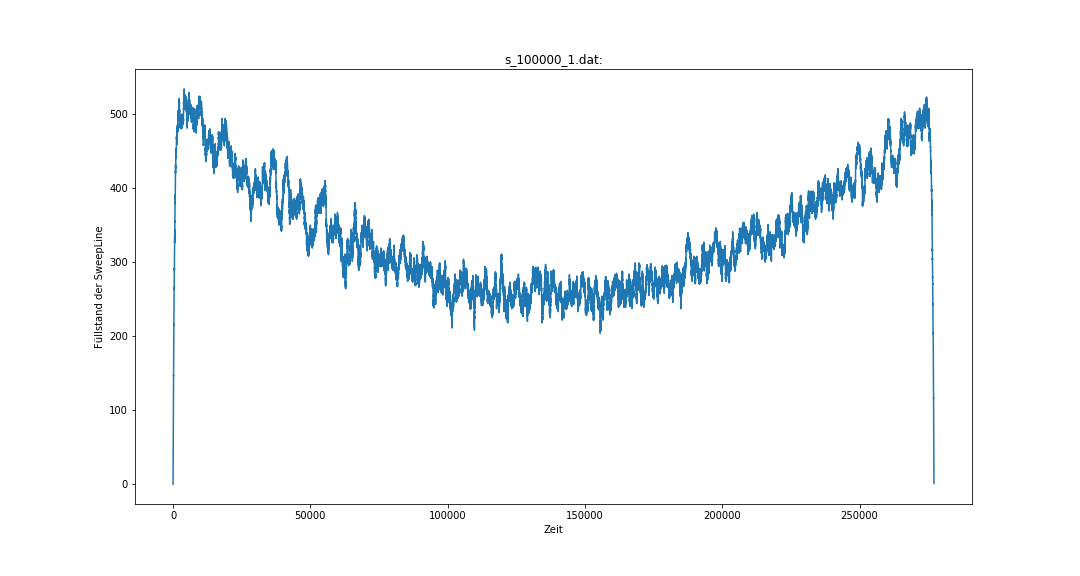
\includegraphics[width=\textwidth]{s100000+1.png}
		\end{minipage}
		\caption{Füllstand der Sweepline über die Zeit}
		\label{fullstand}
	\end{figure}
	
	\begin{thebibliography}{00}
		\bibitem{b2}https://docs.oracle.com/javase/8/docs/api/java/util/PriorityQueue.html
		\bibitem{b1}https://docs.oracle.com/javase/7/docs/api/java/util/TreeMap.html
	\end{thebibliography}
	
	
	
	\section{Anhang}

	Berechnung der Fläche eines Bundeslandes:
	\begin{lstlisting}[basicstyle=\tiny]
	public double calculateArea(){
		double sum = 0;
		for(Polygon p : areas){
			boolean isInside = false;
			for(Polygon p2 : areas){
				//Check if Hole
				if(!p.equals(p2) && p.isPolygonInside(p2) ){ 
					isInside = true;
					break;
				}   
			}
			if(isInside)
				sum -= Math.abs(p.calculateArea());
			else
				sum += Math.abs(p.calculateArea());
		}
		return sum;
	}
	\end{lstlisting}	

\end{document}
